\documentclass[utf8x, 12pt]{G7-32} 
\sloppy

% Настройки стиля ГОСТ 7-32
% Для начала определяем, хотим мы или нет, чтобы рисунки и таблицы нумеровались в пределах раздела, или нам нужна сквозная нумерация.

%\EqInChapter % формулы будут нумероваться в пределах раздела
%\TableInChapter % таблицы будут нумероваться в пределах раздела
%\PicInChapter % рисунки будут нумероваться в пределах раздела

% Добавляем гипертекстовое оглавление в PDF
\usepackage[
bookmarks=true, colorlinks=true, unicode=true,
urlcolor=black,linkcolor=black, anchorcolor=black,
citecolor=black, menucolor=black, filecolor=black,
]{hyperref}

% Изменение начертания шрифта --- после чего выглядит таймсоподобно.
% apt-get install scalable-cyrfonts-tex

\IfFileExists{cyrtimes.sty}
    {
        \usepackage{cyrtimespatched}
    }
    {
        % А если Times нету, то будет CM...
    }

\usepackage{graphicx}   % Пакет для включения рисунков
\DeclareGraphicsExtensions{.jpg,.pdf,.png}
% С такими оно полями оно работает по-умолчанию:
% \RequirePackage[left=20mm,right=10mm,top=20mm,bottom=20mm,headsep=0pt]{geometry}
% Если вас тошнит от поля в 10мм --- увеличивайте до 20-ти, ну и про переплёт не забывайте:
\geometry{right=20mm}
\geometry{left=30mm}



% Произвольная нумерация списков.
\usepackage{enumerate}

\setcounter{tocdepth}{3} %Подробность оглавления
%4 это chapter, section, subsection, subsubsection и paragraph
%3 это chapter, section, subsection и subsubsection
%2 это chapter, section, и subsection
%1 это chapter и section
%0 это chapter.



\begin{document}

\frontmatter 
\begin{center} 

\large САНКТ-ПЕТЕРБУРГСИЙ ГОСУДАРСТВЕННЫЙ ПОЛИТЕХНИЧЕСКИЙ УНИВЕРСИТЕТ

\large Кафедра Компьютерных Систем и Программных Технологий \\[4.5cm] 

\huge ОТЧЕТ \\[0.6cm] % название работы, затем отступ 0,6см
\large по лабораторной работе №1\\
\large Тема: <<Основные виды анализа аналоговых электронных устройств в среде проектирования Cadence Allegro>>\\
\large Дисциплина: <<Автоматическое проектирование аналоговых цифровых устройств>>\\[2.7cm]

\end{center} 

\begin{flushright}
Выполнили: студенты гр. 53501/2 \\
Пономарев М.A \\
Федоров Е.М \\[1.2cm]

Преподаватель \\
Балтруков Н.Н
\end{flushright}


\vfill 

\begin{center} 
\large Санкт-Петербург \\
2015
\end{center} 

\thispagestyle{empty}

\thispagestyle{empty}
\setcounter{page}{0}
\tableofcontents
\clearpage
\mainmatter



\chapter{Задание}

Спроектировать логическое устройство, позволяющее определять, делится ли без остатка или нет $m$--разрядное число $x$, записанное в двоичной системе счисления

\begin{equation}
x = \underbrace{a_1 \quad a_2 \quad \quad a_3 \quad \dots \quad a_m}
\end{equation}
\bigskip


 ,где  $a_i$ --- i--ый разряд числа, $m$ --- количество разрядов.




\chapter{Решение}

\section{Алгоритм решения}

Алгоритм решения задачи основан на признаках деления чисел в двоичной системе счисления. Так для того, чтобы число делилось на 3, знакопеременная сумма цифр должна делиться на 3 без остатка. Приведем пример:

\begin{equation} \label{eq:ex}
\begin{split}
&75_{10} = 1001011_2{}\\
&1+0-0+1-0+1-1=0
\end{split}
\end{equation}

Число в выражении~(\ref{eq:ex}) делится на три. 
\bigskip

Разумно предположить, что нам понадобиться счетчик для хранения текущего значения при вычислении знакопеременной суммы. В теории эта сумма может быть сколь угодно большой, но в силу той особенности, что каждое третье число делится на три нам необходимо хранить только значения в диапазоне от 0 до 2. Хранить значения будем с помощью двух разрядов. Ниже представлена таблица с возможными принимаемыми значениями счетчика:

\begin{table}[hhh!]
	\begin{center}
		\begin{tabular}{|c|c|}
		\hline
		Десятичн. & Двоичн.\\
		\hline
		0 & 100 \\
		1 & 010 \\
		2 & 001 \\
		\hline
		\end{tabular}
	\end{center}	
\end{table}


Положим, наше число $x$ состоит из $m$ разрядов. Тогда
\begin{equation} \label{eq:ex2}
x = \underbrace{a_1 \quad a_2 \quad \dots \quad a_n \quad a_{n+1} \quad \dots \quad a_m}
\end{equation}

\bigskip

Разобьем задачу на фиксированный количество шагов. Каждый шаг будет состоять из фиксированного количества действий, а именно:
\begin{enumerate}
	\item Прибавляем значение $a_n$ к счетчику.
	\item Вычитаем значение $a_{n+1}$ из счетчика.
\end{enumerate}

\newpage

Для решения нам понадобится два логических блока, назовем их SUM и SUB. Приведем схему, реализующую шаг алгоритма:

\begin{figure}[hhh!]
\begin{center}
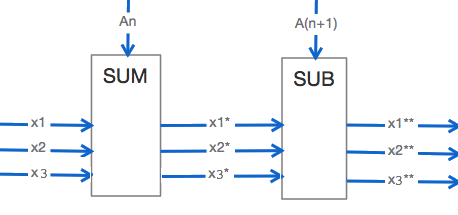
\includegraphics[width=14cm]{img/shema}
\end{center}
\vspace{-5mm}\caption{Схема реализации $i$-го шага алгоритма}
\end{figure}



\newpage

\section{Вспомогательные логические блоки}

\subsection{Блок для прибавления к счетчику разряда}

\begin{itemize}
	\item Переменные:
		\begin{itemize}
			\item $a_n$ --- прибавляемое число
			\item $x_1$, $x_2$, $x_3$  --- входные значения
			\item $y_1$, $y_2$, $y_3$ --- выходные значения
		\end{itemize}
			
\end{itemize}

\bigskip
Таблица истинности:

\begin{table}[hhh!]
	\begin{center}
		\begin{tabular}{|ccc|c||ccc|}
		\hline
		$x_1$ & $x_2$ & $x_3$ & $a_n$ & $y_1$ & $y_2$ & $y_3$\\
		\hline
		1 & 0 & 0 &		0 &		 1 & 0 & 0  \\
		0 &	1 & 0 &		0 &		 0 & 1 & 0 \\
		0 & 0 & 1 &		0 &		 0 & 0 & 1 \\
		\hline
		1 &	0 & 0 &		1 &		 0 & 1 & 0 \\
		0 &	1 & 0 &		1 &		 0 & 0 & 1 \\	
		0 &	0 & 1 &		1 &		 1 & 0 & 0 \\
		\hline
		\end{tabular}
	\end{center}	
\end{table}

\begin{figure}[hhh!]
\begin{center}
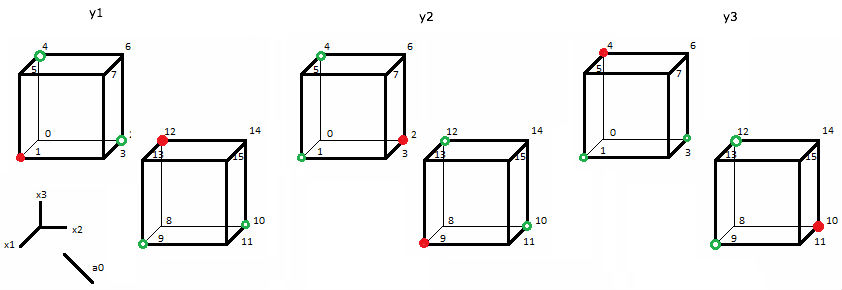
\includegraphics[width=16cm]{img/sum_kubs}
\end{center}
\vspace{-5mm}\caption{Минимизация с помощью гиперкуба}
\end{figure}

\begin{itemize}
	\item Логические функции:
	\begin{itemize}
		\item $y_1 = x_1 \overline{a_n} + x_3 a_n = \overline{\overline{x_1 \overline{a_n}} \, \overline{x_3 a_n}}$
		\item $y_2 = x_2 \overline{a_n} + x_1 a_n = \overline{\overline{x_2 \overline{a_n}} \, \overline{x_1 a_n}}$
		\item $y_3 = x_3 \overline{a_n} + x_2 a_n = \overline{\overline{x_3 \overline{a_n}} \, \overline{x_2 a_n}}$
	\end{itemize}
\end{itemize}

\newpage

\begin{figure}[hhh!]
\begin{center}
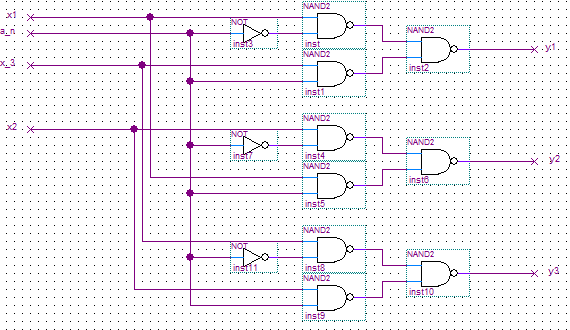
\includegraphics[width=14cm]{img/SUM}
\end{center}
\vspace{-5mm}\caption{Логическая схема блока суммирования}
\end{figure}

\newpage

\subsection{Блок для вычитания из счетчика разряда}

\begin{itemize}
	\item Переменные:
		\begin{itemize}
			\item $a_n$ --- вычитаемое число
			\item $x_1$, $x_2$, $x_3$ --- входные значения
			\item $y_1$, $y_2$ $y_3$ --- выходные значения
		\end{itemize}

\end{itemize}

\bigskip 
Таблица истинности:

\begin{table}[hhh!]
	\begin{center}
		\begin{tabular}{|ccc|c||ccc|}
		\hline
		$x_1$ & $x_2$ & $x_3$ & $a_n$ & $y_1$ & $y_2$ & $y_3$\\
		\hline
		1 & 0 & 0 &		0 &		 1 & 0 & 0  \\
		0 &	1 & 0 &		0 &		 0 & 1 & 0 \\
		0 & 0 & 1 &		0 &		 0 & 0 & 1 \\
		\hline
		1 &	0 & 0 &		1 &		 0 & 0 & 1 \\
		0 &	1 & 0 &		1 &		 1 & 0 & 0 \\	
		0 &	0 & 1 &		1 &		 0 & 1 & 0 \\
		\hline
		\end{tabular}
	\end{center}	
\end{table}


\begin{itemize}
	\item Логические функции:
	\begin{itemize}
		\item $y_1 = x_1 \overline{a_n} + x_2 a_n = \overline{\overline{x_1 \overline{a_n}} \, \overline{x_2 a_n}}$
		\item $y_2 = x_2 \overline{a_n} + x_3 a_n = \overline{\overline{x_2 \overline{a_n}} \, \overline{x_3 a_n}}$
		\item $y_3 = x_3 \overline{a_n} + x_1 a_n = \overline{\overline{x_3 \overline{a_n}} \, \overline{x_1 a_n}}$
	\end{itemize}
\end{itemize}

\begin{figure}[hhh!]
\begin{center}
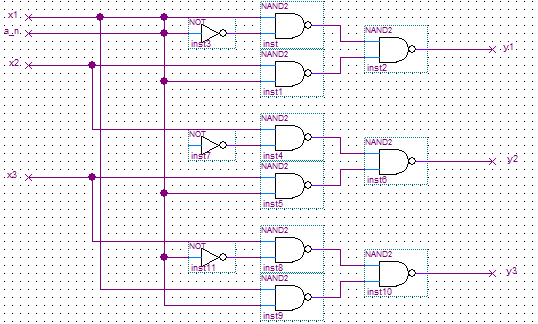
\includegraphics[width=14cm]{img/SUB}
\end{center}
\vspace{-5mm}\caption{Логическая схема блока вычитания}
\end{figure}

\newpage

\subsection{Блок для получения результата}

\begin{itemize}
	\item Переменные:
		\begin{itemize}
			\item $x_1$, $x_2$, $x_3$  --- входные значения
			\item $Y$ --- выходное значение
		\end{itemize}			
\end{itemize}

\bigskip
Таблица истинности:

\begin{table}[hhh!]
	\begin{center}
		\begin{tabular}{|ccc|c|}
		\hline
		$x_1$ & $x_2$ & $x_3$ & $Y$\\
		\hline
		1 & 0 & 0 &		1 \\
		0 & 1 & 0 &		0 \\
		0 & 0 & 1 &		0 \\
		\hline
		\end{tabular}
	\end{center}	
\end{table}

\begin{itemize}
	\item Логическая функция:
	\begin{itemize}
		\item $Y = x_1 \, \overline{x_2} \, \overline{x_3} = \overline{\overline{x_1 \, \overline{x_2} \, \overline{x_3}}}$
	\end{itemize}
\end{itemize}


\begin{figure}[hhh!]
\begin{center}
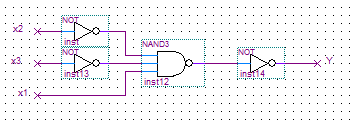
\includegraphics[width=10cm]{img/RES}
\end{center}
\vspace{-5mm}\caption{Логическая схема блока для получения результата}
\end{figure}

\newpage


\section{Результат}


При последовательном соединении спроектированных блоков получаем необходимую реализацию устройства. 

Изначально на входы $x_1$, $x_2$ и $x_3$ подаются нули, последовательно через схему проходят все разряды рассматриваемого числа, на выходе $Y$ получаем <<1>>, если число делиться на 3 или <<0>>, если нет.


\begin{figure}[hhh!]
\begin{center}
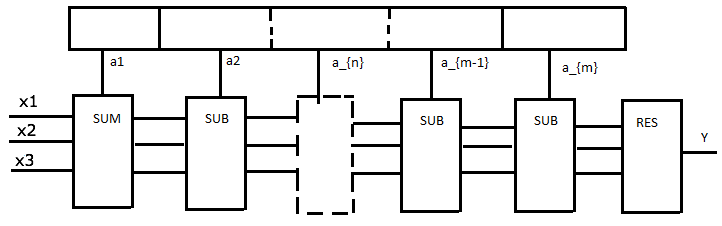
\includegraphics[width=15cm]{img/shema2}
\end{center}
\vspace{-5mm}\caption{Логическая схема результирующего устройства}
\end{figure}



\end{document}
